
\section{Firmware update}
\label{firmware_update}
\index{firmware update}
\index{update}
Firmware updates and a firmware update tool are available for download at
\begin{center}
  \url{http://www.lk-instruments.com}
\end{center}
on the corresponding product website.

In order to update the firmware of the \productNumber ~\productName ~please follow the following procedure:
\begin{itemize}
\item Download the latest firmware for your device and the LK-Instruments Firmware Update Tool.
\item Unpack the downloaded files to a local directory.
\item Connect the device to the power adapter,\\
      but keep it turned off.
\item Connect it to a USB port of your computer.
\item Run the \texttt{LK-Instruments Firmware Update Tool.exe};\\
      a window similar to the one shown in figure~\ref{pic_update_tool} will open.
\item Press and hold the rotary knob.
\item Turn the device on by toggling the power switch.
\item Release the rotary knob.
\item Select the \textsf{COM Port} from the dropdown menu.
\item Select the desired \textsf{Baud Rate} from the dropdown menu.\\
      Typically a baud rate of \texttt{115200} works well, if you have difficulties, try a lower value.
\item Click \textsf{Start Bootloader} and wait until the color of the button changes to green.
\item Click \textsf{Select Flash Hexfile} and point to the downloaded firmware file. It can be recognized by the \texttt{.hex} file ending.
\item Click \textsf{Program Flash} and wait until the color of the button changes to green.
\item Click \textsf{Exit Bootloader} and close the Firmware Update Tool.
\item Open a serial terminal (see \ref{chp:communication_settings}) and send the \texttt{FACTORYRESET} command.


\end{itemize}


\begin{figure}[h]
  \centering
%  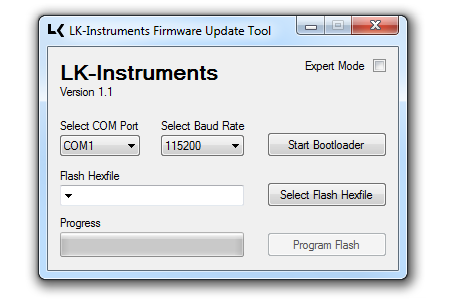
\includegraphics[width=1\textwidth]{./grafiken/update_tool.png}
  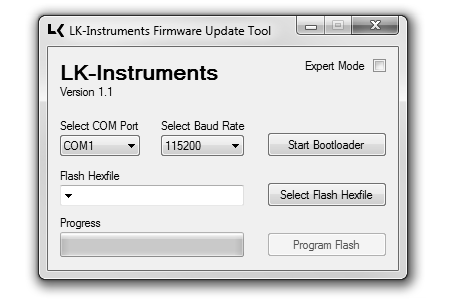
\includegraphics[resolution=96]{./grafiken/update_tool_sw.png}
  \caption[Firmware Update Tool]{LK-Instruments Firmware Update Tool.}
  \label{pic_update_tool}
\end{figure}

